\section{R2G Workflow and Evidence Contracts}
\subsection{Module Boundaries}
R2G comprises four cooperating components: environment provisioning, RTL acquisition, physical implementation and repair, and graph construction. Provisioning resolves tool and platform dependencies and records their configuration. Acquisition handles repository discovery, immutable revisions, synthesis closure, deduplication, and release eligibility. The physical-design component executes ORFS and records implementation and signoff outcomes. The graph component converts these artifacts into stage-aware datasets. Figure~\ref{fig:workflow} summarizes the evidence handoffs.

\begin{figure}[htbp]
\centering
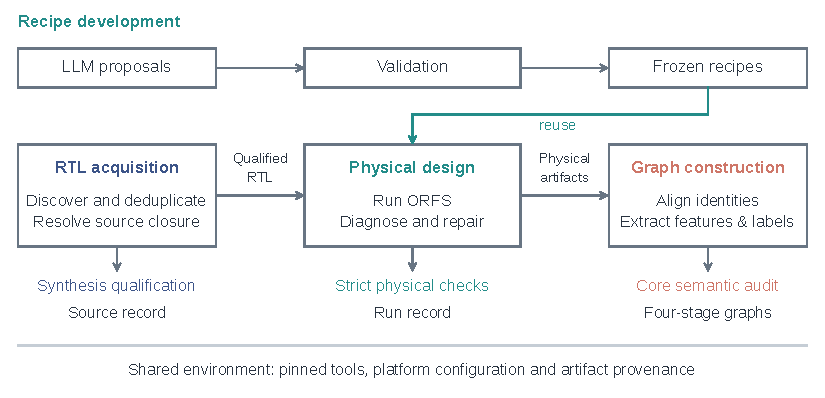
\includegraphics[width=\linewidth]{figures/workflow.pdf}
\caption{R2G workflow and evidence handoffs. A pinned execution environment supports source qualification, physical implementation, and graph construction. Validated repair proposals form frozen recipes for reuse; source, run, and graph records preserve provenance across module boundaries.}
\label{fig:workflow}
\end{figure}

A source record binds repository, commit, top module, compilation inputs, source hashes, and license evidence. A physical run binds configuration, toolchain, stage artifacts, and checking reports. A graph record binds its input artifacts, canonical entity mapping, feature cutoff, label sources, and validation results. These bindings support traceable acceptance decisions and distinguish method failures, unavailable dependencies, and incomplete runs.

The four-stage product incorporates the versioned R2G2.0 builder and recorded integration changes. Its prediction-stage contract is distinct from the five layout views in the prior R2G benchmark~\citep{r2gbenchmark}; code lineage and integration deltas are retained in the artifact documentation.

\subsection{Adaptive Control and Run History}
The operating workflow observes structured candidate records, stage status, failure signatures, physical checks, and graph reports. Admissible decisions include selecting or retrying a candidate, promoting a synthesis-qualified project into physical implementation, applying a scoped repair, resuming an affected stage, scheduling a controlled trial, or escalating a nonconvergent case. Deterministic programs execute these actions and record outcomes. ``Agentic'' describes this observation--decision--execution organization. RTL acquisition and held-out recipe reuse operate without external LLM calls.

The engineer-loop implementation maintains an append-only ledger with pending, flow, signoff, fixing, clean, escalated, and abandoned states. Stage reuse is tied to recorded artifact lineage. Run histories retain failures as well as successes, so recovery does not erase the original outcome. The operational recipe machinery supports candidate, promoted, and shadow states, including evidence-based withdrawal from learned retrieval. Static bootstrap strategies and learned indexed recipes have distinct eligibility paths. The repair experiment evaluates the frozen promotion-and-reuse protocol below.

\subsection{Run-Consistent Dataset Admission}
Physical eligibility and graph validity are distinct requirements. The signoff gate checks backend completion, the required checking reports, and recorded lineage rather than inferring eligibility from a final DEF alone. Its strict mode accepts the exact verdict \texttt{pass}; \texttt{pass\_with\_caveats} belongs to a separate research profile. The required checks and platform capabilities are declared before a campaign.

The complete corpus contract can be expressed as
\begin{equation}
A(d)=Q(d)\land P(d)\land H(d)\land N(d)\land C(d),
\end{equation}
where $Q$ is source qualification, $P$ the declared physical acceptance, $H$ consistent artifact identity and provenance, $N$ native graph validity, and $C$ the implemented core semantic acceptance. Optional label gaps remain explicit in masks and coverage reports; acceptance requires all declared predicates. The conversion experiment evaluates $N$ and $C$ on complete strict-clean physical inputs.

\subsection{Source Qualification}
The acquisition engine discovers repositories, resolves revisions and candidate tops, recovers compilation closure, and forms certified snapshots. The importer checks snapshot and source bindings before synthesis. Deterministic selection limits repository concentration and removes duplicate design families. In the formal acquisition task, each method requests 200 unique designs, with at most four candidates per repository.

Let $q(c)$ indicate whether candidate $c$ passes the frozen qualification rules. These require reproducible source retrieval, a valid top and compilation closure, successful Sky130HD synthesis, a nonempty resolved netlist, $100\leq n_{\mathrm{cells}}<100000$, uniqueness, provenance, and accepted license evidence. The primary yield is
\begin{equation}
Y_{\mathrm{RTL}}=\frac{1}{200}\sum_{c\in\mathcal{S}}q(c),
\end{equation}
where $\mathcal{S}$ is the locked submission. Unfilled slots contribute zero. Submission precision uses $|\mathcal{S}|$ as its denominator and is reported separately. This acquisition gate evaluates synthesis qualification; physical acceptance is evaluated at the subsequent run boundary.

\subsection{Frozen Repair Knowledge}
The repair study separates proposal, validation, and deployment. On the proposal split, LLMs suggest structured configuration actions. Schema and action-policy checks reject invalid parameters, no-ops, and forbidden constraint changes. Admitted candidates must provide useful proposal-split evidence, retain complete provenance, and avoid clean-sentinel regressions. Each executable payload is hashed; exploration outcomes do not themselves count as promotion votes.

After freezing a candidate, formal proposal-split replays and disjoint validation trials provide lifecycle evidence. Let $W$ and $L$ be independent-family wins and losses, $W_v$ validation wins, and $R$ indicate a clean-sentinel regression. The operational promotion rule is
\begin{equation}
\mathrm{promote}(c)=[W\geq2]\land[W>L]\land[W_v\geq1]\land[\neg R].
\end{equation}
Incomplete and inconclusive evidence contributes no promotion vote. Repeated trials from the same RTL family do not provide independent votes. Records with at least two validation wins receive an additional strict-validation-support annotation.

Deployment compares M0 (no learned strategy), M1 (admitted bank in fixed order), M2 (the same bank ranked using A-only evidence), and M3 (promoted recipes only). M1 and M2 attempt at most three candidates per challenge. M2 combines wins, losses, strict-clean outcomes, bounded DRC and WNS gains, and elapsed time in a frozen heuristic; it is not a trained ranking model. M3 abstains when no recipe applies. During held-out deployment, these methods cannot call an LLM, update the bank, or promote a new recipe. The action policy prohibits changing the clock, SDC, footprint, utilization, or signoff check set.

We distinguish overall repair rate $S/N$, policy coverage $C/N$, and conditional success $S/C$. We report all three alongside trial counts to characterize both successful reuse and policy abstention.

\subsection{Four Prediction-Stage Graphs}
For design $d$, the graph builder constructs
\begin{equation}
G_{d,s}=(V_d,E_d,X_{d,s},Y_d,M_d),
\end{equation}
where $V_d$ and logical relations $E_d$ are defined by the canonical post-synthesis netlist. Node types are gates, pins, nets, and I/O pins; core relations are gate--pin membership, pin--net connectivity, and I/O--net connectivity. Features $X_{d,s}$ obey the stage cutoff. Shared post-route labels $Y_d$ retain physical units and explicit validity masks $M_d$.

\begin{table}[htbp]
\caption{Prediction stage and permitted physical inputs. All stages share post-route supervision, which is excluded from encoder inputs.}
\label{tab:cutoff}\centering
\begin{tabular}{lll}\toprule
Graph & Input cutoff & Physical features\\\midrule
Floorplan & Post-synthesis & None\\
Placement & Post-floorplan & Die, I/O, fixed macros\\
CTS & Post-placement & Trusted placement geometry\\
Route & Post-CTS & Trusted CTS geometry\\\bottomrule
\end{tabular}
\end{table}

The node universe remains fixed across stages. A synthesis gate removed by backend optimization remains represented with invalid physical-placement information. Physical net changes are aligned to the canonical topology rather than silently replacing it. Label values satisfy $\mathrm{isfinite}(Y_d)=M_d$; unavailable measurements remain missing, not zero. Timing and RC relations are supervision-only. Their presence as stored relations does not authorize their use in message passing. Geometry relations are permitted only at the CTS and route prediction cutoffs.

\textbf{Joining physical evidence to canonical entities.} R2G uses native Yosys parsing to elaborate bit-level connectivity and normalize escaped identifiers. Assembly joins features and labels by instance, instance--pin, net, and I/O identities, checking key sets before assigning tensor rows and edge indices. Physical extraction then preserves the meaning of each source: routed DEF segments provide wirelength in micrometers after DBU conversion; SPEF names and capacitance units map ground capacitance to canonical nets in pF; STA endpoints map setup/hold slack to canonical pins in ns. These joins carry validity and provenance into the graph. A missing measurement remains masked rather than becoming a zero-valued training target. This design makes topology, physical features, and supervision refer to the same circuit entities.

\subsection{Independent Acceptance Checks}
Native validation checks the output contract, immutable configuration, and structural consistency. An additional oracle checks seven groups: alignment, causal restrictions, identity, labels, masks, numerical features, and topology. Identity and core connectivity are compared with native Yosys parsing. Coordinate checks use OpenDB, LEF, and the permitted DEF. Physical-label checks use independently available route, SPEF, and timing endpoints with frozen tolerances.

For an evaluated design, semantic usability requires native acceptance and a pass in every implemented core group. Each check records pass, fail, or unassessable status. The causal group checks prohibited early features and supervision payloads; label checks report independently matched values and coverage. Semantic usability refers to this implemented core audit.
